\documentclass{beamer}
\usepackage{graphicx}
\usepackage{tikz}
\usetikzlibrary{shapes,arrows}
\usepackage{tikz}
\usetheme{default}
%\usecolortheme{seahorse}
  \setbeamertemplate{footline}[page number]
\usepackage{multirow}
\setbeamertemplate{navigation symbols}{}
\setbeamertemplate{frametitle}[default][center]
\setbeamerfont{frametitle}{shape=\scshape}

\usepackage{xcolor}

\usepackage[flushleft]{threeparttable}

{\title{\textsc{Likelihoods and Bayes} \\ \tiny (See Statistics)}
\author{Trevor Gallen}
\date{}
\begin{document}
\renewcommand*{\inserttotalframenumber}{\pageref{lastframe}}

\begin{frame}
\titlepage
\end{frame}

%\begin{frame}
%\frametitle[alignment=center]{Before we start...}
%\begin{itemize}
%\item Federico Ciliberto
%\bigskip
%\item Bresnahan \& Reiss
%\bigskip
%\item Dentists
%\bigskip
%\item Work together
%\bigskip
%\item Incompletes...Oct 21 vs. Oct 25.
%\end{itemize}
%\end{frame}

\begin{frame}
\frametitle[alignment=center]{Example}
\begin{itemize}
\item Take a two-state Markov chain, in which you observe the following data:
$$X_t=\{2,2,2,2,2,2,2,2,2,2,2,2,2,1,1,2,2,2,2,2,1\}$$
\bigskip
\item Say we wanted to estimate the markov process:
$$\pi=\left[\begin{array}{cc}p_{11} & 1-p_{11} \\ 1-p_{22} & p_{22}\end{array}\right]$$
\item How do we do it? (What is your estimate?)
\end{itemize}
\end{frame}

\begin{frame}
\frametitle[alignment=center]{Maximum Likelihood}
\begin{itemize}
\item We can write down the likelihood of seeing each type of transition:
\begin{align*}
\mathcal{L}_{1\rightarrow 1} & =p_{11}\\
\mathcal{L}_{1\rightarrow 2} & =p_{12}\\
\mathcal{L}_{2\rightarrow 1} & =p_{21}\\
\mathcal{L}_{2\rightarrow 2} & =p_{22}\\
\end{align*}
Or:
$$\mathcal{L}=\prod_{i=1}^T (\mathcal{L}_{1\rightarrow 1})^{x_{11}}(\mathcal{L}_{1\rightarrow 2})^{x_{12}}(\mathcal{L}_{2\rightarrow 1})^{x_{21}}(\mathcal{L}_{2\rightarrow 2})^{x_{22}}$$
\end{itemize}
\end{frame}

\begin{frame}
\frametitle[alignment=center]{Maximum Likelihood}
\begin{itemize}
\item The likelihood:
$$\mathcal{L}=\prod_{i=1}^T (p_{11})^{x_{11}}(1-p_{11})^{x_{12}}(1-p_{22})^{x_{21}}(p_{22})^{x_{22}}$$
\item Taking logs:
\begin{align*}
\log\mathcal{L} & =\sum_{i=1}^T x_{11}\log(p_{11})+x_{12}\log(1-p_{11})\\
 & +x_{21}\log(1-p_{22})+x_{22}\log(p_{22})
 \end{align*}
\item Is this all we can do? \uncover<2->{(Hint: no.)}
\bigskip
\item<3-> The first observation gives us data!

\end{itemize}
\end{frame}


\begin{frame}
\frametitle[alignment=center]{Better Maximum Likelihood}
\begin{itemize}
\item The likelihood:
\begin{align*}
\log\mathcal{L} & =\sum_{i=1}^T x_{11}\log(p_{11})+x_{12}\log(1-p_{11})\\
 & +x_{21}\log(1-p_{22})+x_{22}\log(p_{22})
 \end{align*}
\bigskip
\item Denote a dummy for the first observation as $x^{[1]}$ or $x^{[2]}$, depending on the value:
\begin{align*}
\log\mathcal{L} & =\sum_{i=1}^T x_{11}\log(p_{11})+x_{12}\log(1-p_{11})\\
 & +x_{21}\log(1-p_{22})+x_{22}\log(p_{22}) \\
 & +x^{[1]}\left(\frac{1-p_{22}}{2-p_{11}-p_{22}}\right)+x^{[2]}\left(\frac{1-p_{11}}{2-p_{11}-p_{22}}\right)
 \end{align*}
 \item Why?
\end{itemize}
\end{frame}


\begin{frame}
\frametitle[alignment=center]{Results}
\begin{itemize}
\item We could do things closed form (how?)
\bigskip
\item Or numerically (see Markov.m)
\bigskip
\item What else can we do?
\end{itemize}
\end{frame}

\begin{frame}
\frametitle[alignment=center]{Bayes Rule}
$$P(A|B)=\frac{P(A)P(B|A)}{P(B)}$$
\end{frame}

\begin{frame}
\frametitle[alignment=center]{More Fun with Markovs}
\begin{itemize}
\item Now imagine we didn't observe the states $x_t$ directly, but observed some noise process $y_t$
\bigskip
\item If state $x_t=1$, then $y_t\sim\mathcal{N}(\mu_1,\sigma_1^2)$
\bigskip
\item If state $x_t=2$, then $y_t\sim\mathcal{N}(\mu_2,\sigma_2^2)$
\bigskip
\item To skip annoying notation for the first step, let's say we knew the first state but from then on out we knew nothing else.
\end{itemize}
\end{frame}

\begin{frame}
\frametitle[alignment=center]{Example}
$$x_1=1$$
$$\pi=\left[\begin{array}{cc}0.9 & 0.1 \\ 0.95 & 0.05\end{array}\right]$$
$$y_t|x_t=1\sim\mathcal{N}(0,10)$$
$$y_t|x_t=2\sim\mathcal{N}(1,4)$$
$$P(x_t|y_t)=\frac{P(x_t)P(y_t|x_t)}{P(y_t)}$$
 These types of models are called ``Regime Switching" models\\
 \ \\
See Markov.2
\end{frame}

\begin{frame}
\frametitle[alignment=center]{Example}
\begin{figure}
\centering
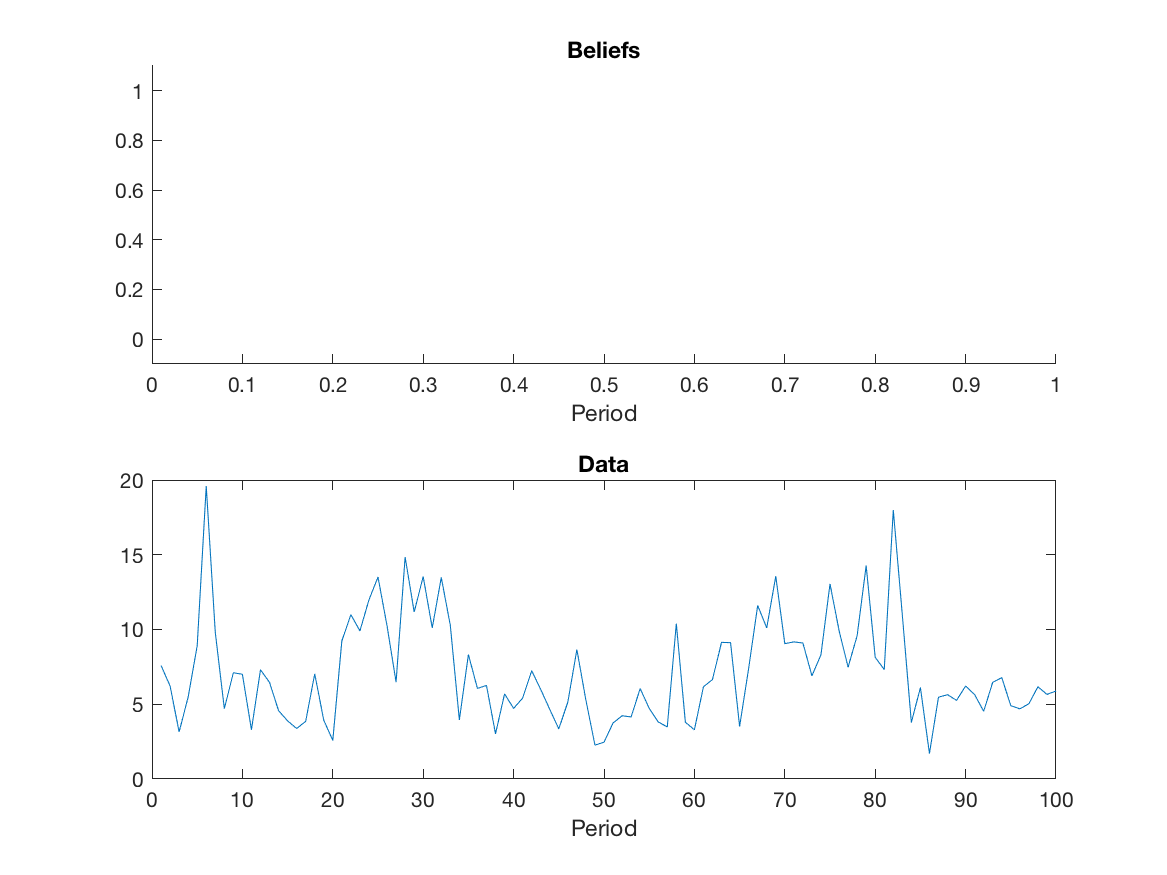
\includegraphics[scale=0.5]{Markov1.png}
\end{figure}
\small
When are we in which state?   $y_t|x_t=1\sim\mathcal{N}(0,10)$, $y_t|x_t=2\sim\mathcal{N}(1,4)$
\end{frame}

\begin{frame}
\frametitle[alignment=center]{Example}
\begin{figure}
\centering
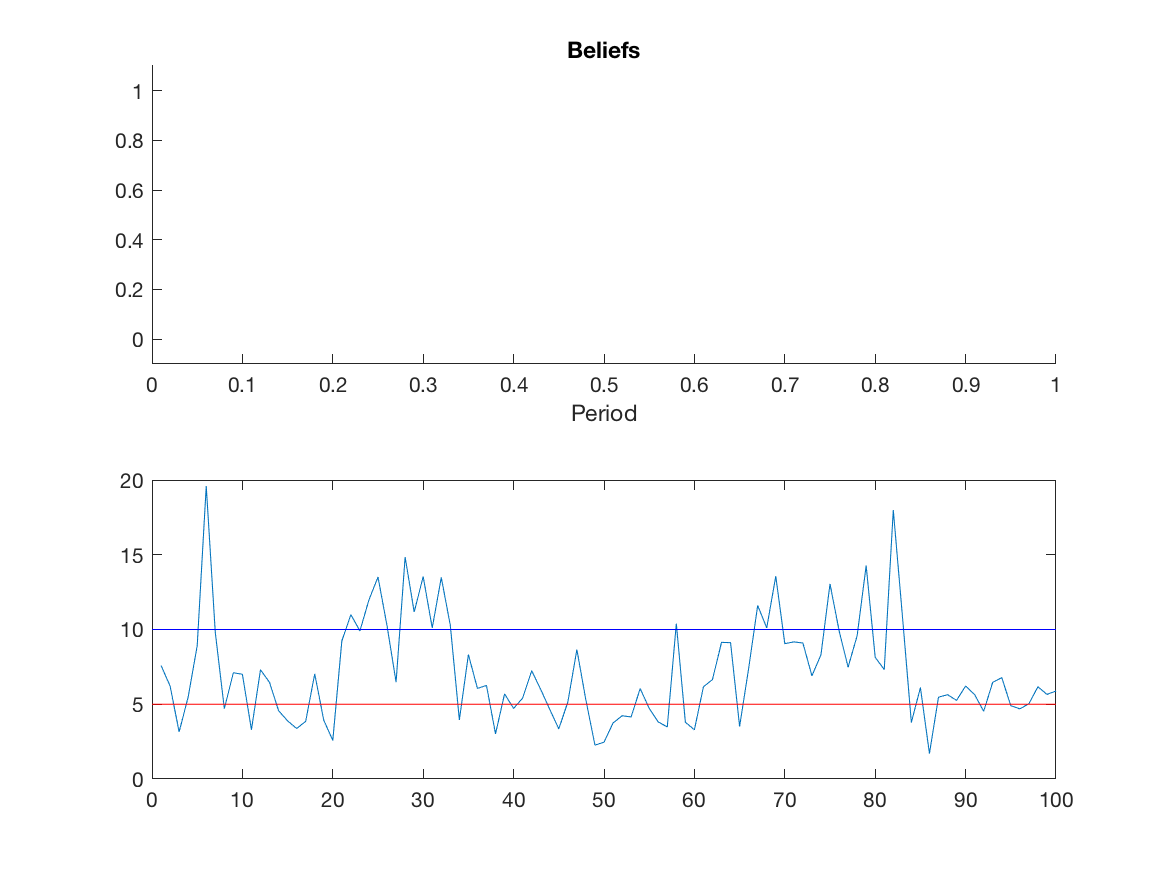
\includegraphics[scale=0.5]{Markov2.png}
\end{figure}
Graphing the means is relevant
\end{frame}

\begin{frame}
\frametitle[alignment=center]{Example}
\begin{figure}
\centering
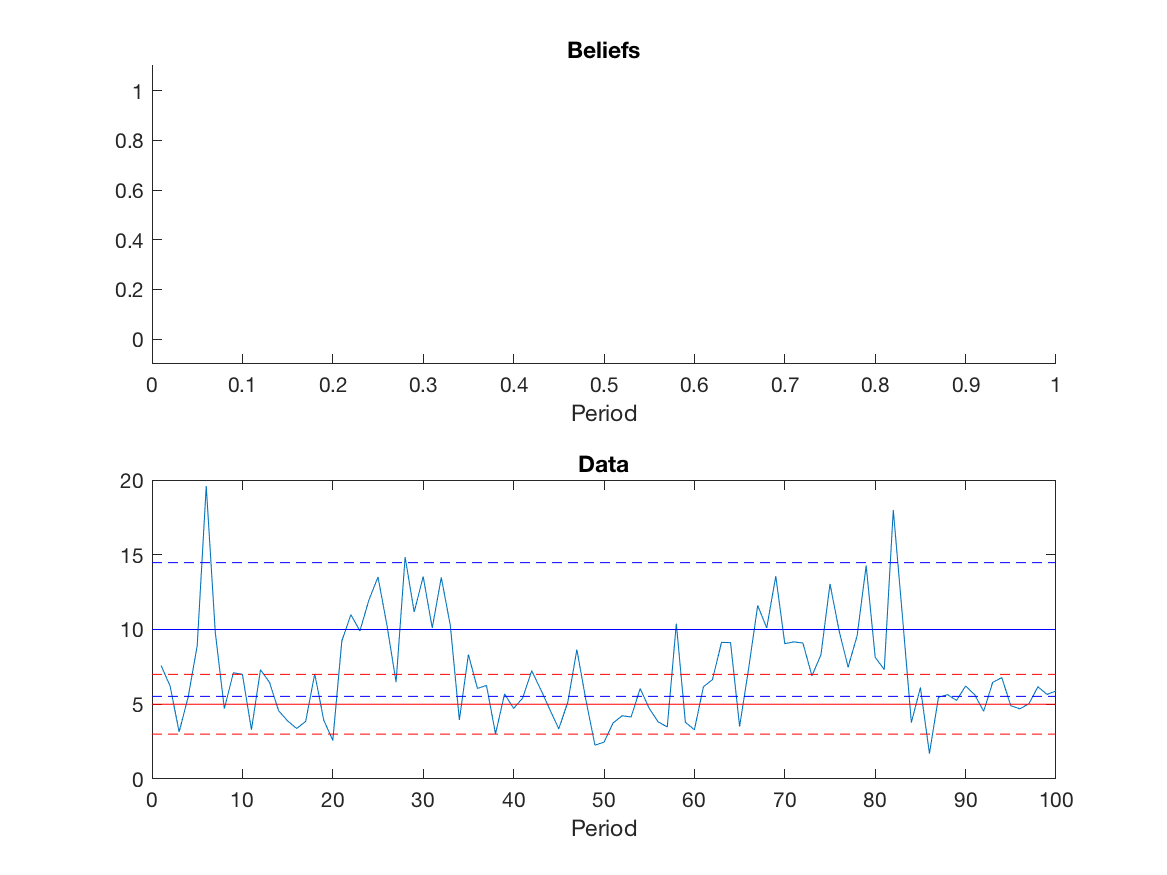
\includegraphics[scale=0.5]{Markov3.png}
\end{figure}
Graphing the 2sd interval is relevant
\end{frame}

\begin{frame}
\frametitle[alignment=center]{Example}
\begin{figure}
\centering
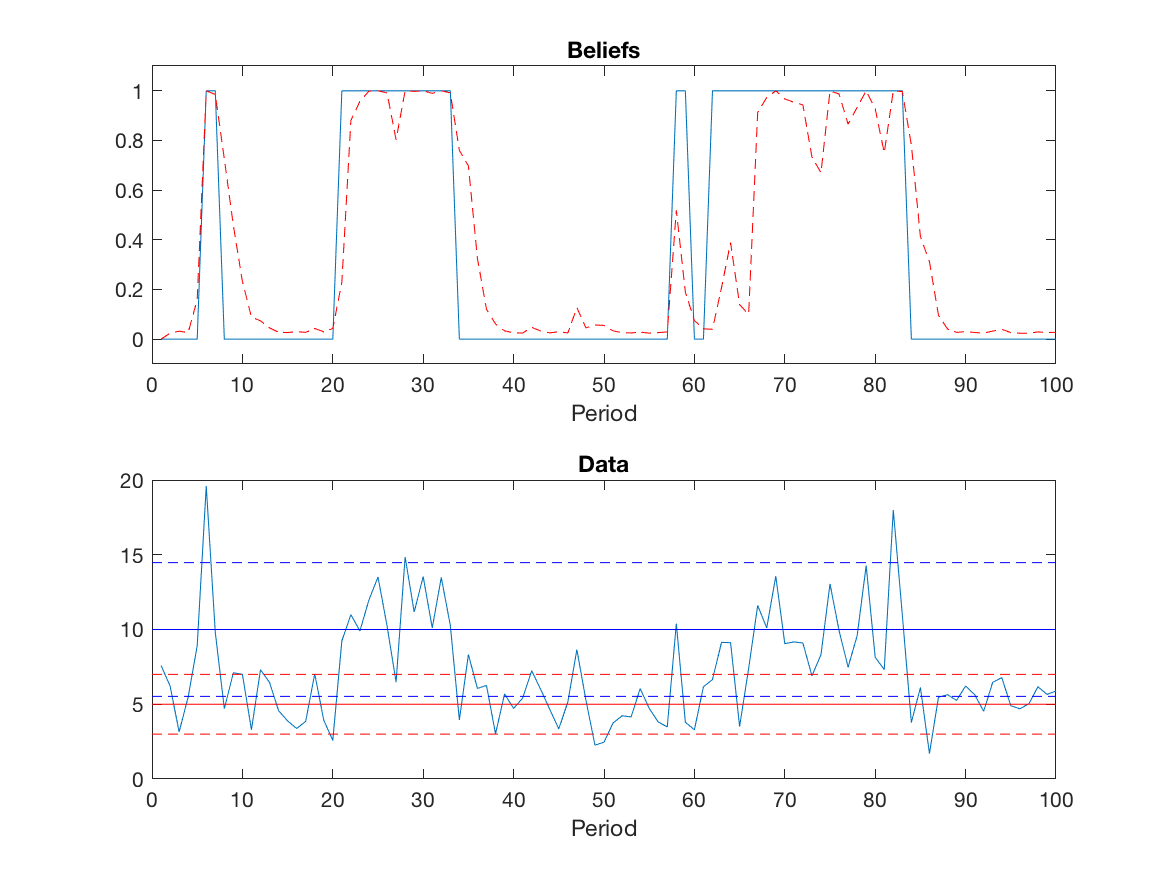
\includegraphics[scale=0.5]{Markov4.png}
\end{figure}
\end{frame}

\begin{frame}
\frametitle[alignment=center]{Example}
\begin{figure}
\centering
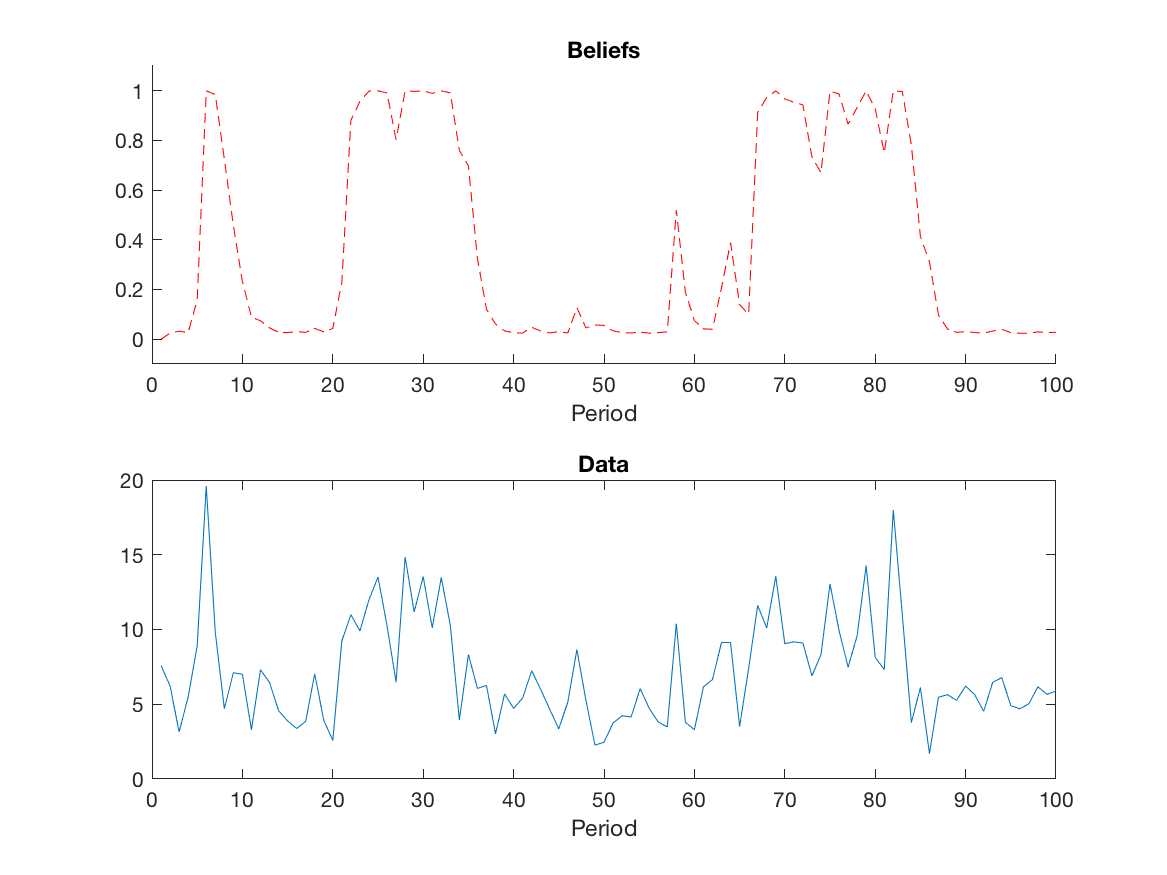
\includegraphics[scale=0.5]{Markov5.png}
\end{figure}
\end{frame}

\begin{frame}
\frametitle[alignment=center]{Example}
\begin{figure}
\centering
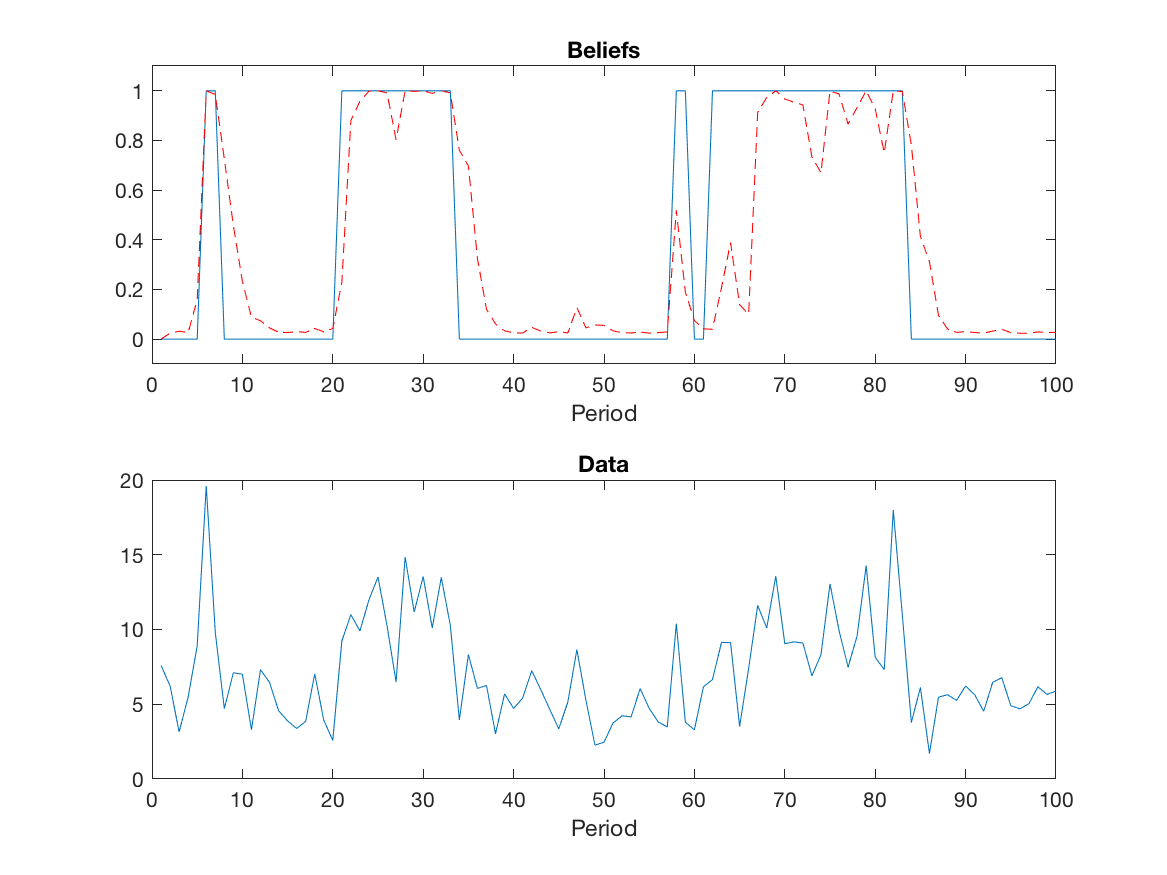
\includegraphics[scale=0.5]{Markov6.png}
\end{figure}
\end{frame}

\begin{frame}
\frametitle[alignment=center]{Kalman Filter: Motivation}
\begin{itemize}
\item Life is full of scenarios in which we see a \emph{signal} about some true underlying process but never observe the truth
\bigskip
\begin{itemize}
\item Missiles
\bigskip
\item Polls
\bigskip
\item Recessions
\bigskip
\item Economic variables
\bigskip
\end{itemize}
\item We typically have some belief of what the underlying object is, where it's going to go, and get some signal related to the object
\bigskip
\item How do we put all our information together?
\end{itemize}
\end{frame}

%\begin{frame}
%\frametitle[alignment=center]{Kalman Filter: Preview to Lemma}
%\begin{itemize}
%\item If $x$ and $y$ are jointly normally distributed 
%\begin{itemize} 
%\item Mean zero 
%\item Variances $\sigma_x^2$, $\sigma_y^2$, 
%\item Covariance $\sigma_{xy}^2$
%\end{itemize}
%\item Then the best fit of $x$ given $y$ comes from the regression:
%$$E(x|y)=\frac{\sigma_{xy}^2}{\sigma_y^2}y$$
%$$Var(x|y)=\sigma_{x}^2-\frac{\sigma_{xy}^2}{\sigma_y^2}\sigma_{xy}^2$$
%\end{itemize}
%\end{frame}

\begin{frame}
\frametitle[alignment=center]{Kalman Filter: Preview to Lemma}
Let $X$ explain $Y$:
$$Y=X\beta+\epsilon$$
Then:
$$\hat{\beta}=(X'X)^{-1}X'Y$$
And:
$$\hat{Y}=X\beta$$
So:
\begin{align*}
Var(Y-\hat{Y}|X) & =Var(Y-X\beta|X)\\
 & =Var(Y|X)+\beta^2\underbrace{Var(X|X)}_{0}-2\beta Cov(Y, X|X))\\
  & =Var(Y|X)-2\beta \frac{\beta}{Var(X)}\\
  & =Var(Y|X)+2\beta^2 Var(X)^{-1}\\
\end{align*}
\end{frame}

\begin{frame}
\frametitle[alignment=center]{Kalman Filter: Lemma$^*$}
If:
$$\left[\begin{array}{c}X \\ Y\end{array}\right]\sim\mathcal{N}\left(\left[\begin{array}{c}0 \\ 0\end{array}\right],\left[\begin{array}{cc}S_{XX'}  & S_{XY'} \\ S_{YX'} & S_{YY'}\end{array}\right]\right)$$
Then:
$$Y|X\sim\mathcal{N}\left(S_{XY'}S_{XX'}^{-1}X,S_{YY'|X}\right)$$
Where, letting $A=S_{XY'}S_{XX}^{-1}$
$$S_{YY'|X}=S_{YY'}-S_{XY'}S_{XX}^{-1}S_{YX'}=S_{YY'}-AS_{XX'}^{-1}A'$$
Matrix analogue of previous slide:
$$Var(Y-\hat{Y}|X)=Var(Y|X)+2\beta^2 Var(X)^{-1}$$
\ \\
In other words, our expectation of $X$ given $Y$ comes from a regression, and our conditional variance is our unconditional variance minus the regression coefficient squared times the variance of our signal.
\ \\
\footnotesize
\ \\
$^*$ This and the next two slides are inspired by Harald Uhlig's notation \& wonderful slides.
\end{frame}


\begin{frame}
\frametitle[alignment=center]{Kalman Motivation}
\begin{itemize}
\item What if you observe some \textbf{possibly noisy} vector of values \textcolor{red}{Y} and want to use them to track some \textbf{possibly moving} vector of values \textcolor{blue}{$\xi$}?
\begin{itemize}
\item Bayesian Estimation: \textcolor{red}{Data} and \textcolor{blue}{Coefficents}
\bigskip
\item Polling: \textcolor{red}{Poll} and \textcolor{blue}{Latent Preferences}
\bigskip
\item Permanent Income: \textcolor{red}{period income and consumption} and \textcolor{blue}{Agent beliefs about permanent income}
\bigskip
\item Ballistic missiles, cars: \textcolor{red}{noisy GPS signal} and \textcolor{blue}{actual location}
\end{itemize}
\bigskip
\item Want to combine noisy observations, unobservable moving due to some law of motion (with noise)
\bigskip
\item This is the Kalman Filter 
\end{itemize}
\end{frame}

\begin{frame}
\frametitle[alignment=center]{Intuition/Shape of Kalman Algorithm}
\begin{itemize}
\item Start with beliefs (mean, variance) about $\xi$ this period (not conditional on information this period)
\bigskip
\item We therefore have beliefs about what $Y$ will be (both itself noisy + don't know $\xi$ in truth)
\bigskip
\item Observe $Y$
\bigskip
\item Degree to which we are surprised by $Y$, plus how much we trust it, determines how we change our beliefs about mean and variance of $\xi$ (conditional on information this period)
\bigskip
\item Now we have (mean, variance) beliefs about today conditional on data today
\bigskip
\item Forecast (mean, variance) beliefs about tomorrow using law of motion
\bigskip
\item Repeat
\end{itemize}
\end{frame}





\begin{frame}
\frametitle[alignment=center]{Kalman System}
\begin{itemize}
\item You have an observation equation:
$$\textcolor{red}{Y_t}=H_t\textcolor{blue}{\xi_t}+\epsilon_t\ \ \ \ \ \epsilon_t\sim\mathcal{N}\left(0,\Sigma_t\right)$$
\item And a state equation:
$$\xi_{t+1}=F_{t+1}\xi_t+\eta_{t+1}\ \ \ \ \ \eta_{t+1}\sim\mathcal{N}\left(0,\Phi_{t+1}\right)$$
\item We assume that $\epsilon_t$ and $\eta_t$ are independent.
\bigskip
\item $Y_t$ is a noisy observation of $\xi_t$, which moves around with noise.
\end{itemize}
\end{frame}

\begin{frame}
\frametitle[alignment=center]{Updating our beliefs}
\begin{itemize}
\item We start with some beliefs from last period about where $\xi$ would be this period (called $\xi_{t|t-1}$).
\bigskip
\item We summarize these as:
$$\xi_{t|t-1}\sim\mathcal{N}\left(\hat{\xi}_{t|t-1},\Omega_{t|t-1}\right)$$
\item We want to look at information today and say what we think $\xi$ is, calling this $\xi_{t|t}$.
\end{itemize}
\end{frame}

\begin{frame}
\frametitle[alignment=center]{First Step: best guess of what the signal will be}
\begin{itemize}
\item We start with beliefs:
$$\xi_t\sim\mathcal{N}\left(\hat{\xi}_{t|t-1},\Omega_{t|t-1}\right)$$
\item And we know, as a law:
$$Y_t=H_t\xi_t+\epsilon_t\ \ \ \ \epsilon_t\sim\mathcal{N}(0,\Sigma_t)$$
\item Then we have our best guess of what $Y$ will be, along with its variance:
$$\hat{Y}_t=H_t\xi_{t|t-1}$$
$$S_{YY|t}=H_t\Omega_{t|t-1}H_t+\Sigma_t$$
\end{itemize}
\end{frame}


\begin{frame}
\frametitle[alignment=center]{Second Step: use surprise info to update prior beliefs}
\begin{itemize}
\item We have our \emph{unexpected} information:
$$\hat{\epsilon}_t=Y_t-\hat{Y}_t$$
\item Then our best fit is, like a regression fit:
$$\hat{\xi}_{t|t}=\hat{\xi}_{t|t-1}+S_{\xi Y'|t}S_{YY'|t}^{-1}\hat{\epsilon}_t$$
\item Where our ``signal" is:
$$S_{\xi Y'|t}=\Omega_{t|t-1}H_t'$$
\item And our beliefs are updated:
$$\Omega_{t|t}=\Omega_{t|t-1}-S_{\xi Y'|t}S_{YY'|t}^{-1}S_{Y\xi'|t}$$
\end{itemize}
\end{frame}

\begin{frame}
\frametitle[alignment=center]{Third Step: use current best beliefs to find tomorrow's best beliefs}
\begin{itemize}
\item We have our beliefs for today, $\hat{\xi}_{t|t}$ and $\Omega_{t|t}$ 
\bigskip
\item We want:
$$\xi_{t+1}\sim\mathcal{N}(\hat{\xi}_{t+1|t},\Omega_{t+1|t})$$
\item Update using the law of motion:
$$\hat{\xi}_{t+1|t}=F_{t+1}\hat{\xi}_{t|t}$$
$$\Omega_{t+1|t}=F_{t+1}\Omega_{t|t}F_{t+1}'+\Phi_{t+1}$$
\end{itemize}
\end{frame}

\begin{frame}
\frametitle[alignment=center]{Summarizing the Kalman Filter}
$$Y_t\sim\mathcal{N}\left(H_t\xi_t,\Sigma_t\right),\ \ \ \ \xi_{t}\sim\mathcal{N}\left(F_{t+1}\xi_t,\Phi_{t+1}\right)$$
\begin{itemize}
\item Given $\xi_t\sim\mathcal{N}(\hat{\xi}_{t|t-1},\Omega_{t|t-1})$,
\begin{enumerate}
\item Forecast $Y_t$ given what you know:
$$\hat{Y}_t=H_t\hat{\xi}_{t|t-1}\ \ \ \ \ \ S_{YY'|t}=H_t\Omega_{t|t-1}H'_t+\Sigma_t$$
\item Update $\xi_t$ given surprise:
$$\hat{\xi}_{t|t}=\hat{\xi}_{t|t-1}+S_{\xi Y'|t}S_{YY'|t}^{-1}(Y_t-\hat{Y}_t)$$
$$\hat{\Omega}_{t|t}=\hat{\Omega}_{t|t-1}+S_{\xi Y'|t}S_{YY'|t}^{-1}S_{\xi Y'|t}$$
Where: $S_{\xi Y'|t}=\Omega_{t|t-1}H_t'$
\item Forecast and set up for tomorrow
$$\hat{\xi}_{t+1|t}=F_{t+1}\hat{\xi}_{t|t}\ \ \ \ \ \Omega_{t+t|t}=F_{t+1}\Omega_{t|t}F'_{t+1}+\Phi_{t+1}$$
\end{enumerate}
\end{itemize}
\end{frame}

\begin{frame}
\frametitle[alignment=center]{Coding it}
See Kalman.m
\end{frame}

\begin{frame}
\frametitle[alignment=center]{Uses}
\begin{itemize}
\item Estimating underlying data, like polls, recessions
\bigskip
\item Alternatively, think of your \emph{regression coefficients} as your unknown $\xi$ and your data as $Y_t$
\bigskip
\item Then for:
$$Y_t\sim\mathcal{N}\left(H_t\xi_t,\Sigma_t\right),\ \ \ \ \xi_{t}\sim\mathcal{N}\left(F_{t+1}\xi_t,\Phi_{t+1}\right)$$
\begin{itemize}
\item $Y_t$ is your dependent variable
\item $H_t$ is your independent variable
\item $\Sigma_t$ is your noise term
\item $F_{t+1}$ is just 1, if your coefficients are constant
\item $\Phi_{t+1}$ is zero, if your coefficients are constant.
\end{itemize}
\item Now you can run Kalman filter point-by-point on your data to uncover your belief\ \emph{distribution} over your coefficients.
\end{itemize}
\end{frame}

\begin{frame}
\frametitle[alignment=center]{Kalman Smoother}
\begin{itemize}
\item Note that your beliefs at any given point are optimal given initial beliefs conditional on information \emph{up to that point}
\bigskip
\item But beliefs about today weren't conditioned on tomorrow's data
\bigskip
\item But tomorrow tells us something about today!
\bigskip
\item Once run Kalman Filter, you have beliefs about $\xi$ conditional on all past data, can run in reverse, condition beliefs about yesterday on today's data
\bigskip
\item This is the Kalman Smoother
\end{itemize}
\end{frame}



\begin{frame}
\frametitle[alignment=center]{One More Example: BVars (DSGE estimation)} 
\begin{itemize}
\item Standard feel of a DSGE estimation:  \textbf{parameters are unknown state}, and \emph{data take place of parameters}
$$\underbrace{\left[\begin{array}{c} c_{t} \\   y_{t} \\ i_t \end{array}\right]}_{Y_t}=\overbrace{\underbrace{\left[\begin{array}{cccccc}   y_{t-1} & 0 & 0 \\ 0 & y_{t-1} & 0 \\ 0 & 0 & y_{t-1}\end{array}\right]}_{H_t}}^{\text{Data!}}\overbrace{\underbrace{\left[\begin{array}{c}   \beta_{1,t } \\ \beta_{2,t } \\ \beta_{3,t }  \end{array}\right]}_{\xi_t}}^{\text{Parameters}}+\left[\begin{array}{c}\epsilon_{1,t} \\ \epsilon_{2,t} \\ \epsilon_{3,t} \end{array}\right]$$
$$\Sigma=\left[\begin{array}{ccc}\sigma^2_{\epsilon_1} & \cdot & \cdot \\ \cdot & \sigma^2_{\epsilon_2} & \cdot \\ \cdot & \cdot & \sigma^2_{\epsilon_3} \end{array}\right]$$

And the ``state equation" is:
$$\left[\begin{array}{c}   \beta_{1,t+1 } \\ \beta_{2,t +1} \\ \beta_{3,t+1 }  \end{array}\right]=\underbrace{\left[\begin{array}{cccc} 1 \\ 1 \\ 1 \end{array}\right]}_{F}\left[\begin{array}{c}   \beta_{1,t } \\ \beta_{2,t } \\ \beta_{3,t}  \end{array}\right]\ \ \ \ \ \Phi = \left[\begin{array}{c}0\end{array}\right]$$
\end{itemize}
\end{frame}


\begin{frame}
\frametitle[alignment=center]{Our use: Insurance}
\begin{itemize}
\item As labor, macro, and public economists, we care about people's lifecycle income paths
\bigskip
\item We know a random walk component is important
\bigskip
\item We know transitory shocks are also important
\bigskip
\item Write down a simple flexible model of income $y_{i,t}$ as the sum of permanent income $z_{i,t}$ and perfectly transitory shock $\epsilon_{i,t}$.
$$y_{i,t}=z_{i,t}+\epsilon_{i,t}$$
\item Where permanent income is subject to a shock $\zeta_{i,t}$
$$z_{i,t}=z_{i,t-1}+\zeta_{i,t}$$
\item Note:  for more about this, read Meghir and Pistaferri (ECMA 2004) or Blundell, Pistiaferri, and Preston (AER 2008)
\end{itemize}
\end{frame}


\begin{frame}
\frametitle[alignment=center]{Our use: Insurance}
\begin{itemize}
\item We can therefore write the \emph{change} in income as:
$$y_{i,t}=z_{i,t}+\epsilon_{i,t}$$
\item If we're interested in what consumption tells us about income, we might also have:
$$c_{i,t}=\phi z_{i,t}+\psi \epsilon_{i,t}+\xi_{i,t}$$
\item Where $\phi$ and $\psi$ are the MPC out of permanent and temporary income changes, respectively.  $\xi_{i,t}$ denotes shocks that change consumption, but not income (such as lifecycle concerns, so it may be common between individuals).  
\bigskip
\item This allows both $y$ and $c$ to tell us about permanent income 
\bigskip
\item Two observations:  income and consumption
\bigskip
\item Two (or three) hidden variables:  ``true" permanent income $z_{i,t}$, transitory income $\epsilon_{i,t}$ and transitory consumption shock $\xi_{i,t}$.
\end{itemize}
\end{frame}

\begin{frame}
\frametitle[alignment=center]{Aside:  What's the motivation?}
\begin{figure}
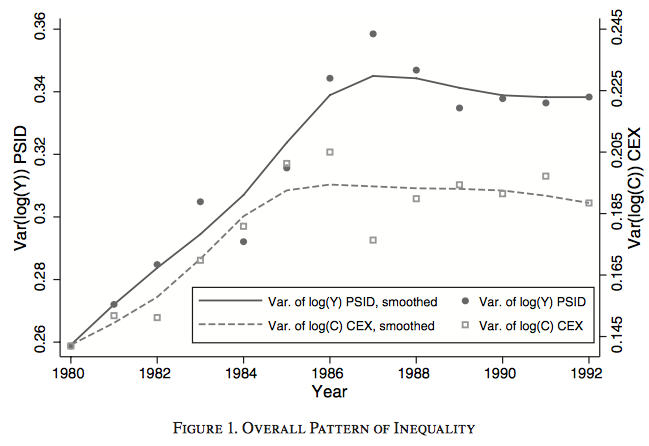
\includegraphics[scale=0.5]{BPP.png}
\end{figure}
Increase in $y$ variance double increase in $c$ variance!
\end{frame}

\begin{frame}
\frametitle[alignment=center]{Aside:  Consumption inequality}
\begin{figure}
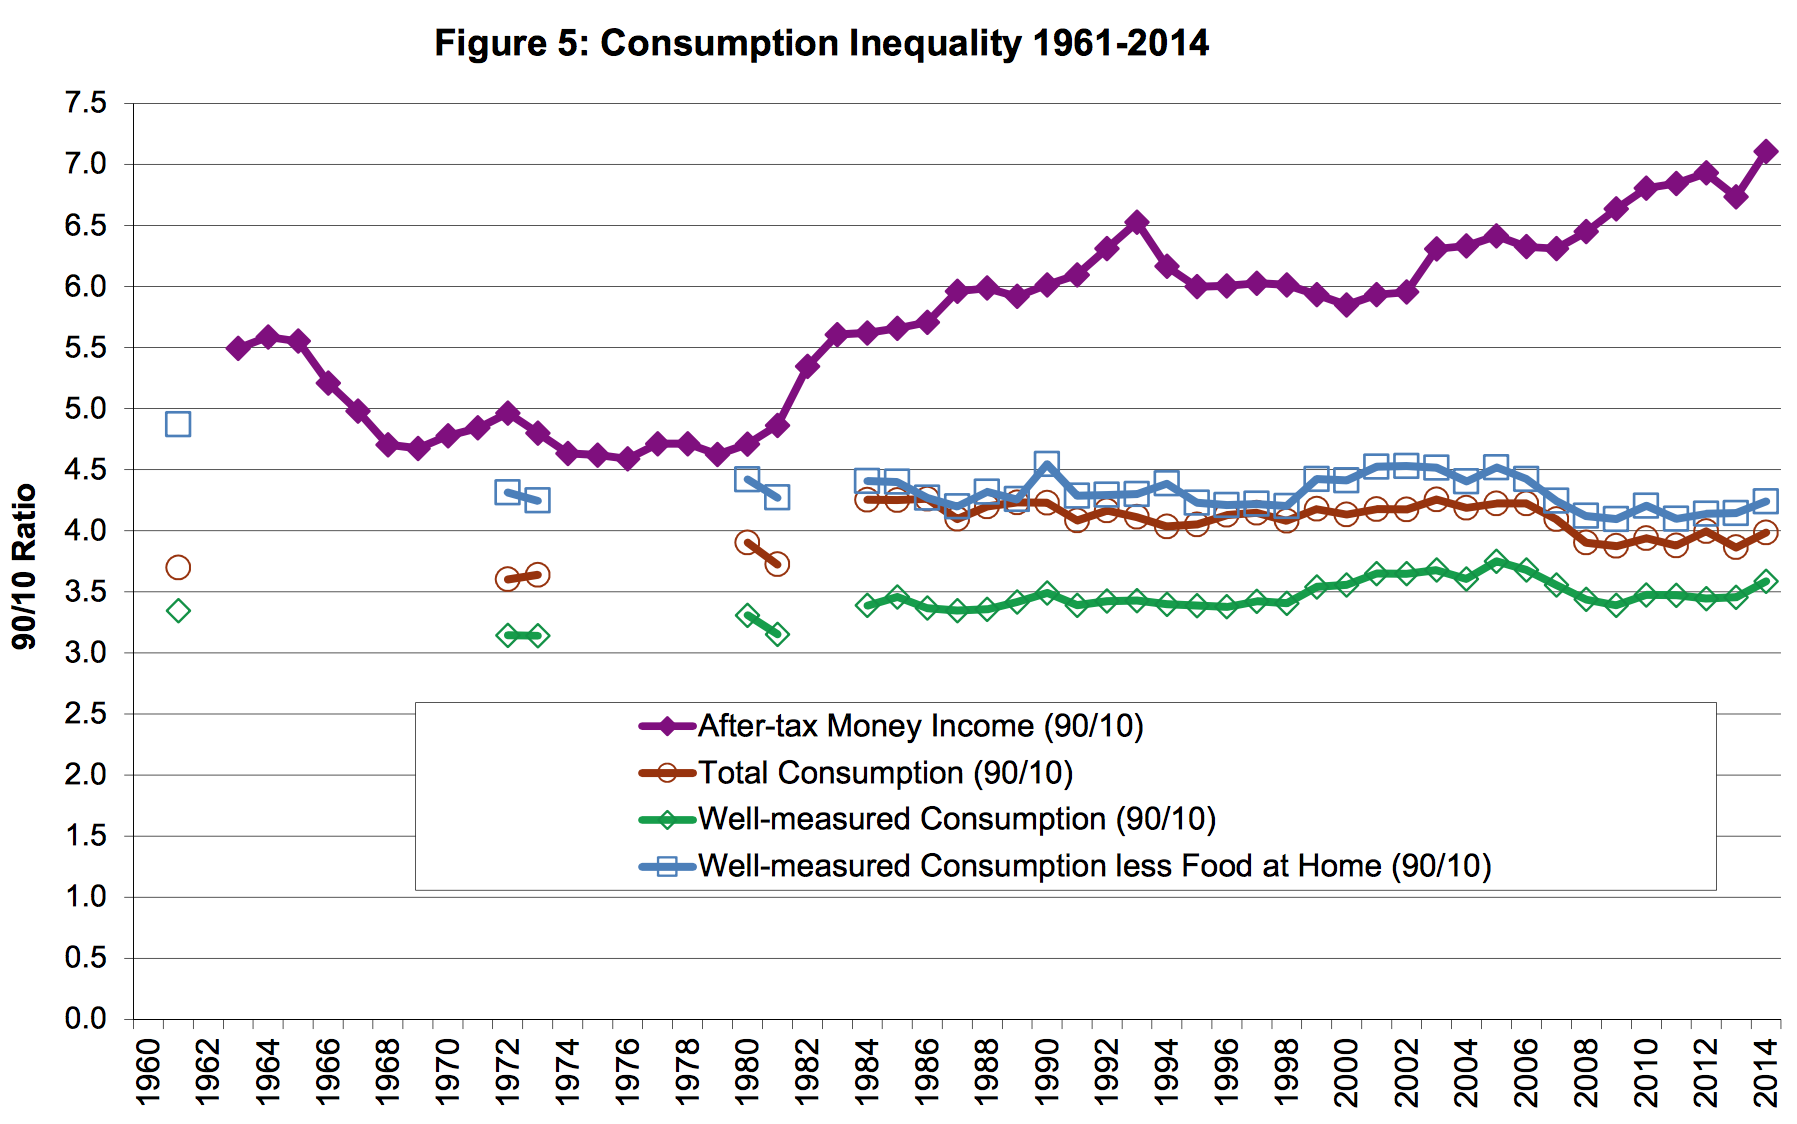
\includegraphics[scale=0.18]{MeyerSullivan2017.png}
\end{figure}
\end{frame}


\begin{frame}
\frametitle[alignment=center]{Insurance: Kalman}
Applying the Kalman Filter's notation for $H$, $F$, $\Sigma$, $\Phi$, $\xi$, and $Y$, above, we can write out the ``observation equation":
$$\underbrace{\left[\begin{array}{c} c_{i,t} \\   y_{i,t} \end{array}\right]}_{Y}=\underbrace{\left[\begin{array}{cccccc}   \phi  \\ 1 \end{array}\right]}_{H}\underbrace{\left[\begin{array}{c}   z_{i,t }  \end{array}\right]}_{\xi_t}+\left[\begin{array}{c}\psi\epsilon_{i,t}+\xi_{i,t} \\  \epsilon_{i,t} \end{array}\right]$$
$$\Sigma=\left[\begin{array}{cc}\psi^2 \sigma^2_\epsilon+\sigma^2_\xi & \psi \\ \psi & \sigma^2\epsilon \end{array}\right]$$

And the ``state equation" is:
$$\left[\begin{array}{c}   z_{i,t+1 }\end{array}\right]=\underbrace{\left[\begin{array}{cccc} 1 \end{array}\right]}_{F}\left[\begin{array}{c}   z_{i,t }\end{array}\right]$$

$$\Phi = \left[\begin{array}{c}\sigma^2_\zeta\end{array}\right]$$
\end{frame}

\begin{frame}
\frametitle[alignment=center]{Identification}
\begin{itemize}
\item But how do we get the parameter values out?  The variances?  
\bigskip
\item Can estimate from conditional moments
\bigskip
\item For instance:
\small
\begin{align*}
E(\Delta y_{t}\Delta y_{t-1}) & = E((\zeta_{i,t}+\Delta \epsilon_{i,t})(\zeta_{i,t-1}+\Delta \epsilon_{i,t-1}))\\
& = E(\zeta_{i,t}\zeta_{i,t-1}+\Delta \epsilon_{i,t}\zeta_{i,t-1}+\zeta_{i,t}\Delta \epsilon_{i,t-1}+\Delta \epsilon_{i,t}\Delta \epsilon_{i,t-1})\\
& = E((\epsilon_{i,t}-\epsilon_{i,t-1})(\epsilon_{i,t-1}-\epsilon_{i,t-2}))\\
& = E(-\epsilon_{i,t-1}\epsilon_{i,t-1})\\
& = -\sigma^2_\epsilon\\
\end{align*}
\item Intuition:  the only reason the change in income today \& change in income yesterday are correlated is the transitory shock, which shows up in both periods (one coming in, the other going out).
\end{itemize}
\end{frame}

\begin{frame}
\frametitle[alignment=center]{Our use}
\begin{itemize}
\item Similiarly:  
\footnotesize
\begin{align*}
E(\Delta c_{t}\Delta c_{t-1}) & = E\left(\left(\phi \zeta_{i,t}+\psi \Delta \epsilon_{i,t}+\Delta \xi_{i,t}\right)\left(\phi \zeta_{i,t-1}+\psi \Delta \epsilon_{i,t-1}+\Delta \xi_{i,t-1}\right)\right)\\
& = E\left(\left(\psi \Delta \epsilon_{i,t}+\Delta \xi_{i,t}\right)\left(\psi \Delta \epsilon_{i,t-1}+\Delta \xi_{i,t-1}\right)\right)\\
& = E(\left(\psi (\epsilon_{i,t}-\epsilon_{i,t-1})+(\xi_{i,t}-\xi_{i,t-1})\right)(\psi (\epsilon_{i,t-1}-\epsilon_{i,t-2})+\\
 & +(\xi_{i,t-1}-\xi_{i,t-2})))\\
& = E\left(\left(-\psi\epsilon_{i,t-1}-\xi_{i,t-1}\right)\left(\psi (\epsilon_{i,t-1}-\epsilon_{i,t-2})+(\xi_{i,t-1}-\xi_{i,t-2})\right)\right)\\
& = E\left(-\psi^2 \epsilon_{i,t-1}\epsilon_{i,t-1}-\xi_{i,t-1}\xi_{i,t-1}\right)\\
& = -\psi^2\sigma^2_\epsilon-\sigma^2_\xi\\
\end{align*}
\item There are two reasons consumption today and yesterday are correlated.  First, the transitory shock (weighted by $\psi$) increases consumption in the first period relative to the second, in which it falls.  Second, consumption has its own ``transitory" shock, which comes in just as $\epsilon$ did.
\end{itemize}
\end{frame}

\begin{frame}
\frametitle[alignment=center]{Our use}
The identifying equations derived above are summarized in Table \ref{tab:strucest}:
\begin{table}[ht!]
$$
\begin{array}{rcl}
\hline\hline
\text{Data} & & \text{Structural Equation}\\
\hline
E(\Delta y_{i,t}\left(\Delta y_{i,t-1}+\Delta y_{i,t}+\Delta y_{i,t+1}\right)) & = &\sigma^2_\zeta\\
E(\Delta y_{t}\Delta y_{t-1}) & = & -\sigma^2_\epsilon\\
E(\Delta c_{t}\Delta c_{t-1}) & = &-\psi^2\sigma^2_\epsilon-\sigma^2_\xi\\
E(\Delta c_t\Delta y_{t}) & = & \phi \sigma_\zeta^2+2\psi \Delta \sigma_\epsilon^2\\
E(\Delta c_t(\Delta y_{t-1}+\Delta y_{t}+\Delta y_{t+1}))  & = & \phi\sigma^2_\zeta  \\
\hline\hline
\end{array}$$
\caption{This table summarizes the identifying equations for $\sigma^2_\zeta$, $\sigma^2_\xi$, $\sigma^2_\epsilon$, $\phi$, and $\psi$. }
\label{tab:strucest}
\end{table}
\end{frame}

\begin{frame}
\frametitle[alignment=center]{How good is our estimator?}
\begin{table}[ht!]
\centering
\begin{tabular}{lccccc}
\hline\hline
Description & Parm. & Value & Est.  & Est.  & Est. \\
 &  &  & N=10 & N=50 & N=10000\\
\hline
$c$ to a perm. $y$  & $\phi$ & 1 & 1.11 & 0.54 & 1.02\\
$c$ to a trans. $y$  & $\psi$ & 0.1 & 0.33 & 0.09 & 0.10\\
StdDev of trans. $y$  & $\sigma_\epsilon$ & 0.1 & -0.04 & 0.10 & 0.10\\
StdDev of perm. $y$  & $\sigma_\zeta$ & 0.1 & 0.07 & 0.06 & 0.10\\
StdDev of trans. $c$  & $\sigma_\xi$ & 0.1 & 0.05 & 0.08 & 0.11\\
\hline\hline
\end{tabular}
\end{table}
\end{frame}

\begin{frame}
\frametitle[alignment=center]{How good is our estimator?}
\begin{itemize}
\item Once we have the parameters, we can let the Kalman filter rip!  Uncover hidden states.
\begin{figure}[ht!]
\centering
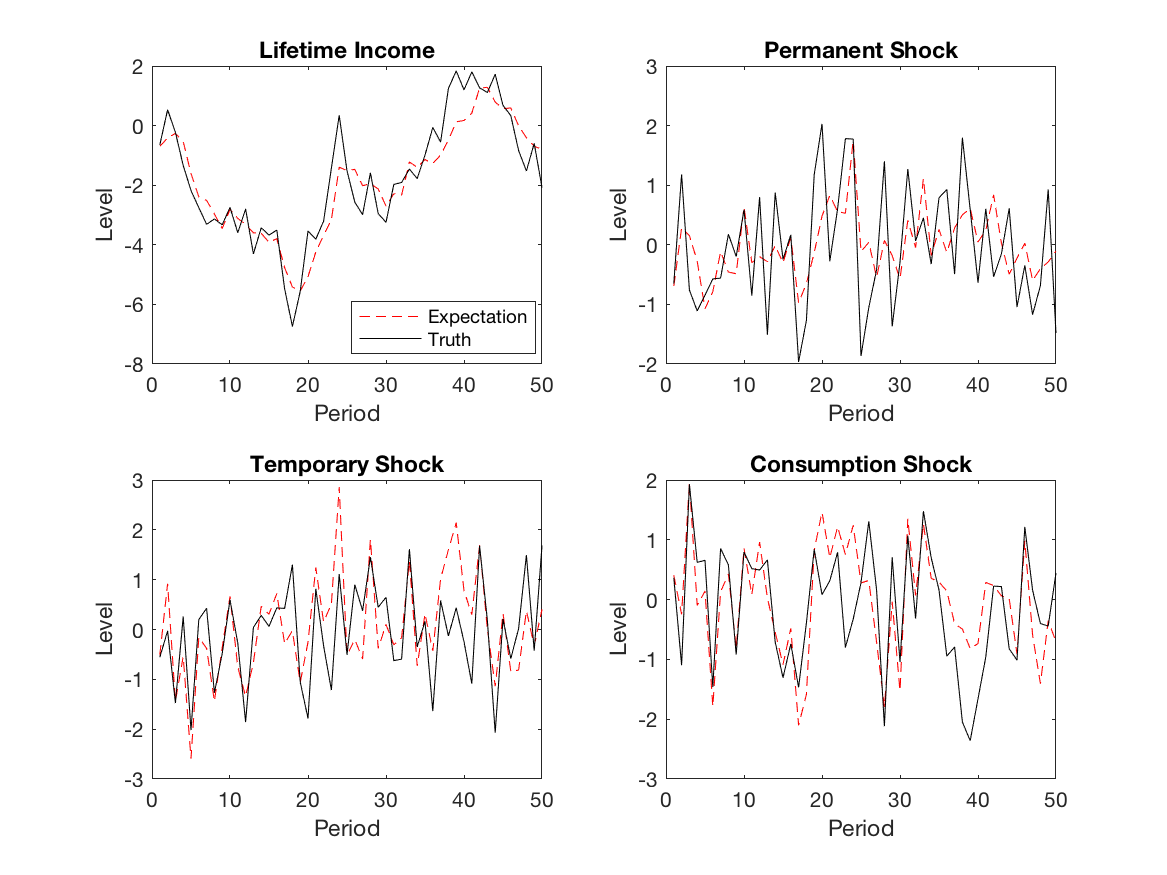
\includegraphics[scale=0.5]{KalmanFilter.png}
\caption{This figure depicts both the true value of four theoretically unknown objects as solid black lines, as well as our Kalman filtered values in dashed red lines.  The four objects are: (1) lifetime income $z_{i,t}$, (2) the permanent shock to income $\zeta_{i,t}$, (3) the temporary shock to income and (4) $\epsilon_{i,t}$, and the temporary consumption shock $\xi_{i,t}$.}
\label{fig:kalfilter}
\end{figure}
\end{itemize}
\end{frame}

\begin{frame}
\frametitle[alignment=center]{How good is our estimator?}
\begin{itemize}
\item Compare belief about permanent shock to permanent shock
\begin{figure}[ht!]
\centering
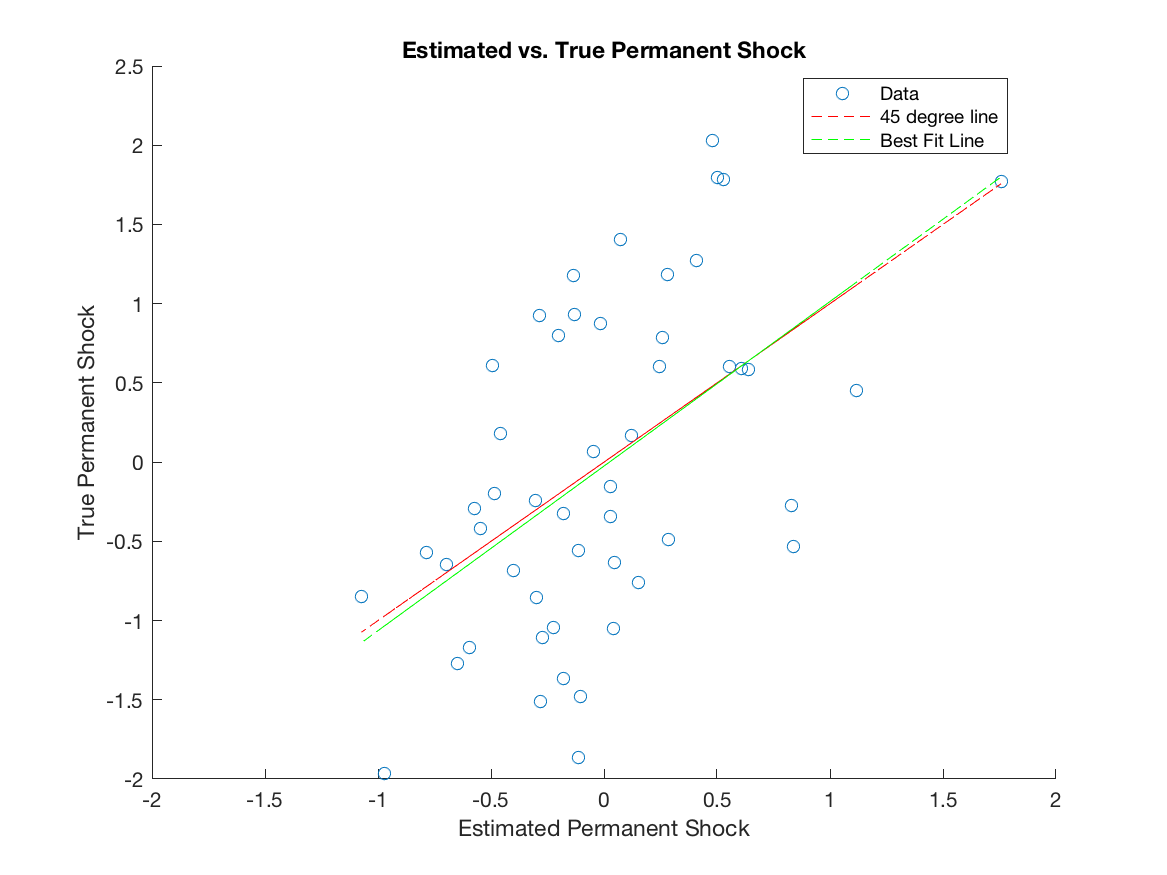
\includegraphics[scale=0.45]{PermShocks.png}
\end{figure}
\item $R^2\approx 0.54$
\end{itemize}
\end{frame}


\begin{frame}
\frametitle[alignment=center]{How good is our estimator?}
\begin{itemize}
\item Remember, these all have standard errors!
\begin{figure}[ht!]
\centering
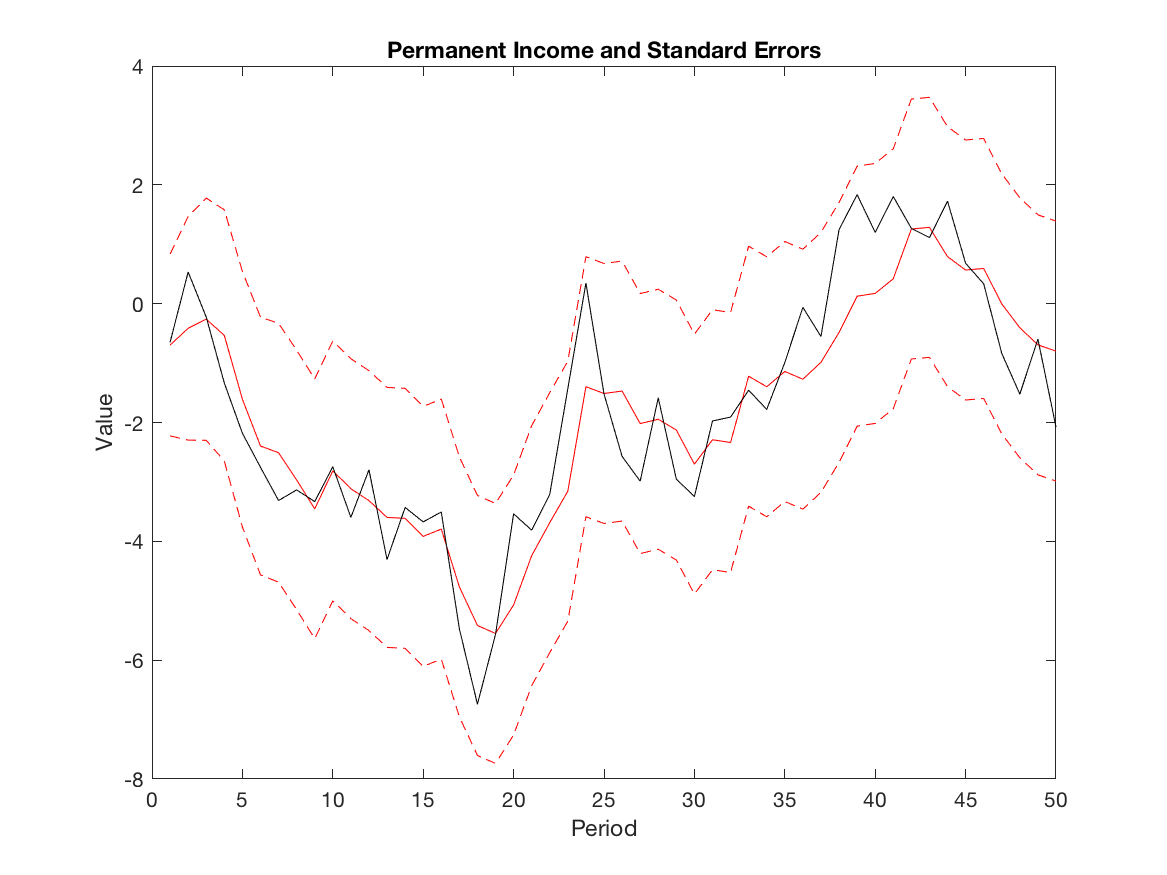
\includegraphics[scale=0.45]{KalmanFilter2.png}
\end{figure}
\item Can run regressions on these, know how to correct for attrition bias!
\end{itemize}
\end{frame}



\begin{frame}
\frametitle[alignment=center]{Concluding Thoughts}
\begin{itemize}
\item If you ever do structural estimation with different, hidden regimes, need to filter
\bigskip
\item If you ever want to (partially) uncover hidden state (such as permanent income) Kalman Filter
\bigskip
\begin{itemize}
\item Note:  might not be super practical in example we gave!
\end{itemize}
\bigskip
\item Very useful in time series estimation
\bigskip
\item Used to estimate most macro models (DSGE)
\end{itemize}
\end{frame}


\end{document}